\section{Patrón de diseño: Modelo Vista Controlador}
El patrón de diseño de software Modelo Vista Controlador se encarga de separar en tres distintos componentes la interfaz de usuario, la lógica de control y los datos de la aplicación. Dichos componentes son:\\

\begin{itemize}
	\item \textbf{Modelo}: es el encargado de los datos que serán manejados en el sistema, contiene los meccanismos de persistencia y la lógica de negocio de estos\cite{mvc}.\\
	
	\item \textbf{Vista}: se encarga de componer la información que será enviada al cliente, así como los mecanismos de interacción con éste\cite{mvc}.
	
	\item \textbf{Controlador}: se encarga de gestionar el flujo de información entre el Modelo y la Vista, es decir, transforma los datos del Modelo para las necesidades de la Vista.
	
\end{itemize}

La Figura \ref{fig:mvc} muestra a grandes razgos un diagrama de como opera el patrón de diseño

\begin{figure}[htbp]
	\begin{center}
		\hypertarget{fig:mvc}{
			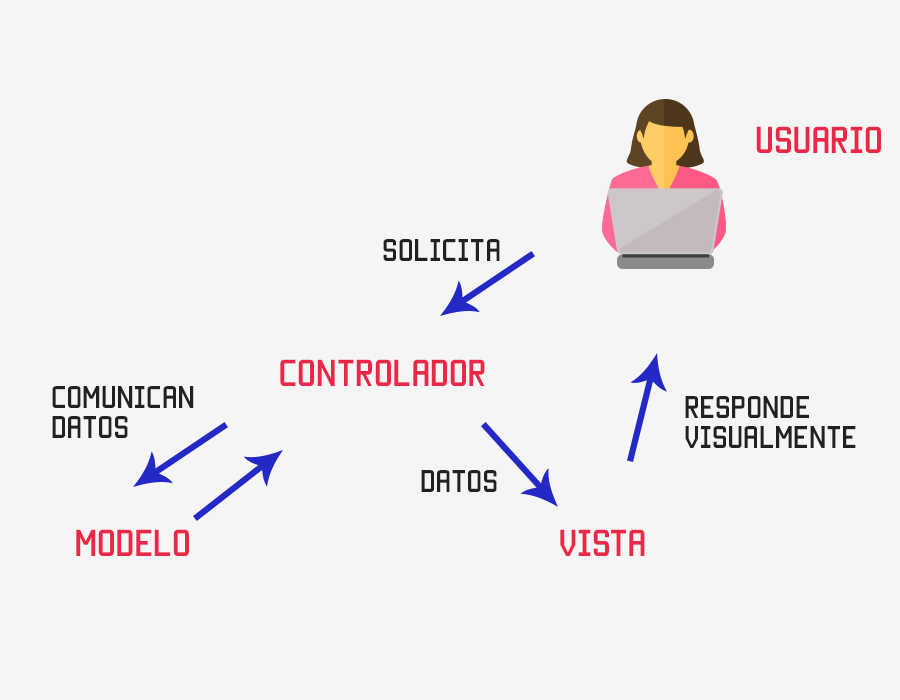
\includegraphics[scale=.3]{propuestaSolicion/turismo/images/mvc}
			\caption{Modelo Vista Controlador\cite{mvcImagen}}
		}
		\label{fig:mvc}
	\end{center}
\end{figure}

\newpage
A continuación se describen las principales responsabilidades de cada uno de los componentes: 

\subsection{Modelo}
\begin{itemize}
	\item Manipular, gestionar y actualizar los datos\cite{mvc2}.
	
	\item Consultas, búsquedas, filtros y actualizaciones de base de datos\cite{mvc2}.
	
	\item Definir las reglas de negocio\cite{mvc2}.
	
\end{itemize}

\subsection{Vista}
\begin{itemize}
	\item Recibir datos del modelo y mostrarlos al usuario (pantallas, ventanas, formularios)\cite{mvc2}.
	
\end{itemize}

\subsection{Controlador}
\begin{itemize}
	\item Recibir instrucciones, atenderlas y procesarlas\cite{mvc2}.
	
	\item Comunicar al Modelo con la Vista\cite{mvc2}.
	
	\item Solicitar datos y manipularlos para ser presentados\cite{mvc2}.
\end{itemize}

\section{Diseño del pratrón Modelo Vista Controlador}

A continuación se detallán los diseños del patrón Modelo Vista Controlador que fueron utilizados para el desarrollo del proyecto. \\

La Figura \ref{fig:MVC} muestra el diseño llevado a cabo para el patrón Modelo Vista Controlador.\\

\begin{figure}[htbp]
	\begin{center}
		\hypertarget{fig:MVC}{
			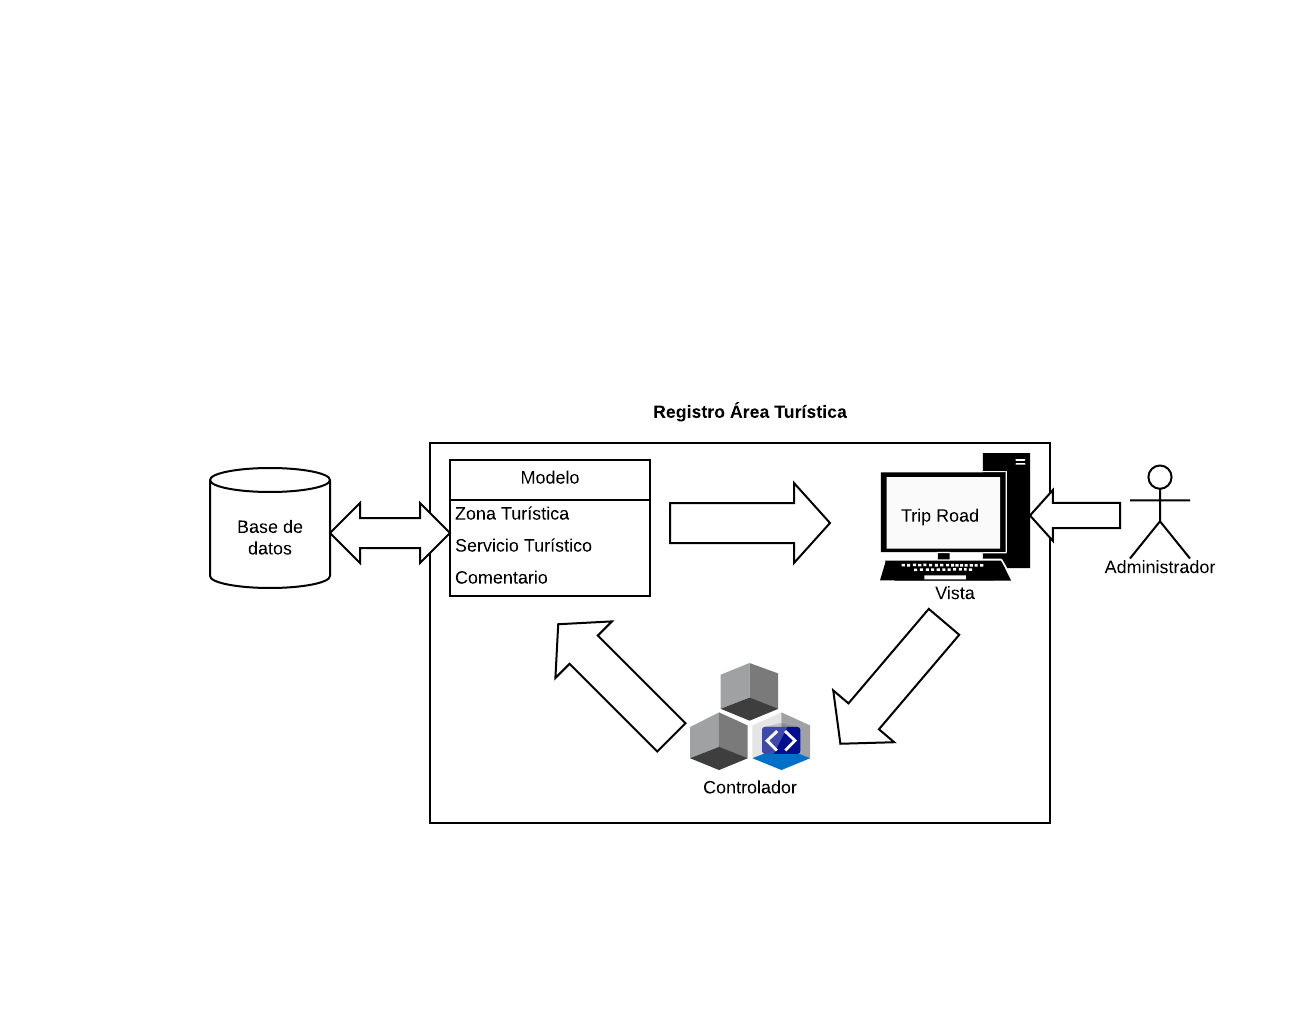
\includegraphics[scale=.7]{propuestaSolicion/turismo/images/MVC2}
			\caption{Diseño del Patrón Modelo Vista Controlador}
		}
		\label{fig:MVC}
	\end{center}
\end{figure}